\section{Terminology}

We refer to the Glossary in the OpenMP standard document~\cite{OpenMP} for the
terms defined there.

This document refers to \emph{contexts} and \emph{handles}.
Contexts are entities that are defined by the debugger, and are opaque
to the OMPD implementation.
Handles are entities that are defined by the OMPD implementation, and
are opaque to the debugger.
The OMPD API contains opaque definitions of debugger contexts
(see Section~\ref{debugger-contexts:sec}) and OMPD handles
(see Section~\ref{ompd-handles:sec}).

Data passed across the interface between the debugger and the
OMPD implementation must be managed to prevent memory leakage.
Space for data may be allocated on the stack, static data areas,
thread local storage, or the heap.
In all cases, the data will be said to have an \emph{owner}
which is responsible for deallocating them when they are
no longer needed.
The owner need not be---in fact in many cases is not---the same component
that allocated the memory.
Where the creating component and owner are different, memory will
usually be allocated on the heap.
The OMPD implementation must not access the heap directly,
but instead it must use the callbacks supplied to it by the debugger.
The specific mechanism that must be used by an owner to deallocate memory will
depend on the entity involved.
Memory management is covered in more detail in
Section~\ref{memory-management:sec}.

All OMPD-related symbols needed by the debugger must have \texttt{C} linkage.

\subsection{OMPD Concepts}
\label{ompd-concepts:sec}

Figure~\ref{ompd-concepts:fig} depicts the OMPD concepts of
\emph{process}, \emph{address space}, \emph{thread}, \emph{image
file}, and \emph{target architecture}, which are defined as follows:

\paragraph{Process}
A process is a collection of one or more threads and address spaces.
The collection may be homogeneous or heterogeneous, containing,
for example, threads or address spaces from host programs or
accelerator devices.
A process may be a ``live'' operating system process,
or a core file.

\paragraph{Thread}
A thread is an execution entity running within a specific address
space within a process.

\paragraph{Address Space}
An address space is a collection of logical, virtual, or physical
memory address ranges containing code, stack, and data. 
The memory address ranges within an address space need not be
contiguous.  
An address space may be segmented, where a segmented address consists
of a segment identifier and an address in that segment. 
An address space has associated with it a collection of image files
that have been loaded into it. 
For example, an OpenMP program running on a system with GPUs may
consist of multiple address spaces: one for the host program and one
for each GPU device. 
In practical terms, on such systems an OpenMP \emph{device} may be
implemented as a CUDA context, which \emph{is} an address space into
which CUDA image files are loaded and CUDA kernels are launched.

\paragraph{Image File}
An image file is an executable or shared library file that is loaded
into a target address space.
The image file provides symbolic debug information to the debugger.

\paragraph{Target Architecture}
A target architecture is defined by the processor (CPU or GPU) and the
Application Binary Interface (ABI) used by threads and address spaces.
A process may contain threads and address spaces for multiple target
architectures.

For example, a process may contain a host address space and threads
for an x86\_64, 64-bit CPU architecture, along with accelerator
address spaces and threads for an
NVIDIA\textsuperscript{\textregistered} GPU architecture or for an
Intel\textsuperscript{\textregistered} Xeon
Phi\textsuperscript{\texttrademark} architecture.

\begin{figure}
  \centering
    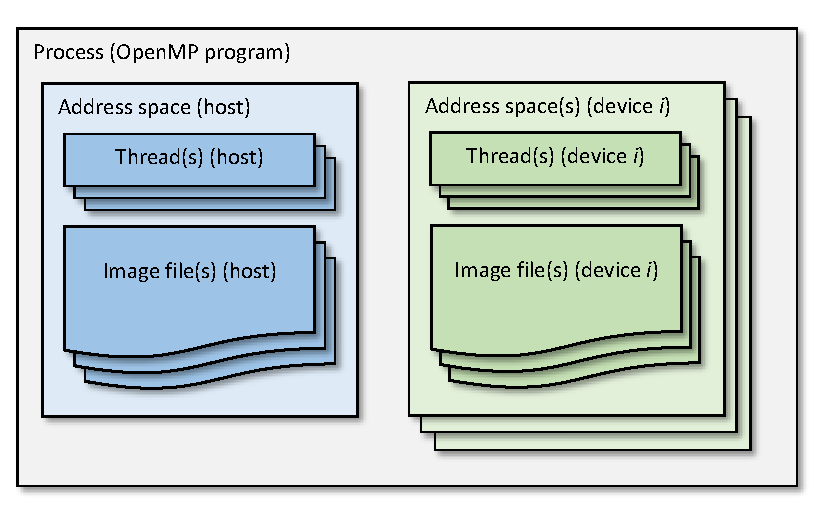
\includegraphics[width=6.0in,natwidth=396,natheight=252]{figures/ompd-concepts.pdf}
  \caption{Key concepts of OMPD}
\label{ompd-concepts:fig}
\end{figure}

\subsection{OMPD Handles}
OMPD handles identify OpenMP entities during the
execution of an OpenMP program.
Handles are opaque to the debugger, and defined internally
by the OMPD implementation.
Below we define these handles and the conditions under which they
are guaranteed to be valid.

\paragraph{Address Space Handle}
The \emph{address space handle} identifies a portion of an instance of
an \emph{OpenMP program} that is running on a host device or a target
device.
The host address space handle is allocated and initialized with the per 
process or core file initialization 
call to \refdef{\texttt{ompd\_process\_initialize}}{process-initialize:def}. 
A process or core file is initialized by passing the host address
space context to that function to obtain an address space handle for
the process or core file.
The handle remains valid until it is released by the debugger.

\begin{notes}
ilaguna: In the description of each handle we say "handle is allocated and 
initialized" to make it clear that the handles interface is callee-allocates, 
not caller-allocates. This seems a bit repetitive. Perhaps we want to make this 
concept clear in a central place (e.g., a subsection) instead of repeating it 
in each handle description.
\end{notes}

The handle is created by the OMPD implementation, which passes ownership
to the debugger which is responsible for indicating when it no longer
needs the handle.
The debugger releases the handle when it calls
\refdef{\texttt{ompd\_release\_address\_space\_handle}}{release-address-space-handle:def}.
The OMPD implementation can use the handle to cache invariant
address-space-specific data (e.g., symbol addresses), and to retain a copy of 
the
debugger's address space context pointer.
The handle is passed into subsequent API function calls.
In the OMPD API, an address space handle is represented by the opaque type
\texttt{ompd\_address\_space\_handle\_t}.
%
\emph{Future versions of this API will support address space handles
for target devices, which will be allocated and initialized by various
OMPD API calls.}

\paragraph{Thread Handle}
The \emph{thread handle} identifies an \emph{OpenMP thread}.
Thread handles are allocated and initialized by various OMPD API calls.
A handle is valid for the life time of the corresponding system thread.
Thread handles are represented by \texttt{ompd\_thread\_handle\_t},
and created by the OMPD implementation which passes ownership to the
debugger which is responsible for indicating when it no longer
needs the handle.
The debugger releases the thread handle by calling
\refdef{\texttt{ompd\_release\_thread\_handle}}{release-thread-handle:def}.

\paragraph{Parallel Handle}
The \emph{parallel handle} identifies an \emph{OpenMP parallel region}.
It is allocated and initialized by various OMPD API calls.
The handle is valid for the life time of the parallel region.
The handle is guaranteed to be valid if at least one thread
in the parallel region is paused, or if a thread in a nested
parallel region is paused.
Parallel handles are represented by the opaque type
\texttt{ompd\_parallel\_handle\_t}, and created by the OMPD implementation
which passes ownership to the debugger which is responsible for
indicating when it no longer needs the handle.
The debugger releases the parallel handle by calling
\refdef{\texttt{ompd\_release\_parallel\_handle}}{release-parallel-handle:def}.

\paragraph{Task Handle}
The \emph{task handle} identifies an \emph{OpenMP task region}.
It is allocated and initialized by various OMPD API calls.
The handle is valid for the life time of the task region.
The handle is guaranteed to be valid if all threads
in the task team are paused.
Task handles are represented by the opaque type
\texttt{ompd\_task\_handle\_t}, and created by the OMPD implementation
which passes ownership to the debugger which is responsible for
indicating when it no longer needs the handle.
The debugger releases the task handle by calling
\refdef{\texttt{ompd\_release\_task\_handle}}{release-task-handle:def}.


\subsection{Debugger Contexts}
Debugger contexts are used to identify a process, address space, or thread 
object
in the debugger.
Contexts are passed from the debugger into various OMPD API calls,
and then from the OMPD implementation back to the debugger's
callback functions.
For example, symbol lookup and memory accesses are done in the ``context''
of a particular address space and possibly thread in the debugger.
Contexts are opaque to the OMPD implementation, and defined by the debugger.

%% \begin{comment} %by Joachim
%% It is possible for the OMPD implementation to ``navigate'' process,
%% address space, and thread object relationships using callback
%% functions.  For example, given a thread context, it is possible to get
%% the address space context for the thread, or the process context
%% containing the thread.
%% 
%% \paragraph{Process Context}
%% The \emph{process context} identifies the debugger object for a process.
%% The debugger owns and initializes the process context.
%% A process context is a \emph{container} for address space and thread
%% contexts.
%% A process \emph{always} contains a host address space bound to a host
%% device.
%% A process \emph{may} contain host threads, device address spaces bound
%% to target devices, and device threads.
%% \end{comment}

\paragraph{Address Space Context}
The \emph{address space context} identifies the debugger object for a
portion of an instance of an \emph{OpenMP program} that is running on
a host or target device.
An address space is contained within a process, and has an associated
target architecture.
The address space context must be valid for the life time of its
associated address space handle.
The host address space context is passed into the process initialization call
\refdef{\texttt{ompd\_process\_initialize}}{process-initialize:def}
to associate the host address space context with the address space handle.
The OMPD implementation can assume that the address space context is valid
until
\refdef{\texttt{ompd\_release\_address\_space\_handle}}{release-address-space-handle:def}
is called for the address space context passed into the initialization routine.

\paragraph{Thread Context}
The \emph{thread context} identifies the debugger object for a thread.
The debugger owns and initializes the thread context.
The OMPD implementation obtains a thread context using the
\texttt{get\_thread\_context} callback.
This callback allows the OMPD implementation to map an operating
system thread ID to a debugger thread context.
The OMPD implementation can assume that the thread context is valid
for as long as the debugger is holding any references to thread handles
that may contain the thread context.

\subsection{Operating System Thread Identifiers}

An operating system thread ID,
%% \refdef{\texttt{ompd\_osthread\_t}}{osthread-kind-t:def},
is the object that allows the debugger and OMPD implementation
to map a thread handle to and from a thread context.
That is, the OS thread ID is the common identifier for a thread
that is visible to both the debugger and the OMPD implementation.
The operating system-specific information is platform dependent,
and therefore is not defined explicitly in this API.
Thus the interface defines
\refdef{\texttt{ompd\_osthread\_kind\_t}}{osthread-kind-t:def}
which identifies what ``kind'' of information an operating system
thread ID represents, such as \texttt{pthread\_t},
lightweight process ID, or accelerator-specific ID.
When an operating system thread ID needs to be passed across
the interface, the caller passes the ``kind'' of the ID,
the size of the ID in bytes, and a pointer to the
operating system-specific information.
The format of the information, such as byte ordering, is that
of the target.
The ID is owned by the caller, which is responsible for its
allocation and deallocation.

%\begin{center}
\begin{notes}
%\sl
JVD: For maximum interoperability, we may want to provide ``advice to
implementers'' to always support the lowest common denominator thread
ID on the platform. For example, using ``LWP IDs'' (gettid()) on Linux
would allow support for debuggers that do not support the
\verb|thread_db| library, thus do not know the \verb|pthread_t| of a
thread.
%\end{center}
\end{notes}